\documentclass[a4paper,man,natbib,floatsintext,noextraspace]{apa6}

\usepackage[english]{babel}
\usepackage[utf8x]{inputenc}
\usepackage{amsmath}
\usepackage{graphicx}
\usepackage[colorinlistoftodos]{todonotes}
\usepackage{apacite}

\title{Development of affordance perception and recalibration}
\shorttitle{Affordance Perception and Recalibration}
\author{John M. Franchak}
\affiliation{University of California, Riverside}

\abstract{Your abstract here.}

\begin{document}
\maketitle

\section{Introduction}

Perceiving affordances means distinguishing which actions are possible given an observer's body size and capabilities \citep{Gibson79}. For example, the affordance for passing through a narrow doorway may be possible for a small child but impossible for a large adult. With \textit{calibrated} affordance perception---that is, perception that is in line with their actual abilities---the child would perceive the doorway as possible to navigate but the adult would not. However, uncalibrated perception may lead the observer to make a poor decision, such as attempting to fit through a doorway that is too small or refusing the walk through a doorway that is sufficiently large. Developmental studies suggest that affordance perception becomes better calibrated through childhood for various actions. Younger children (3-5 years) made large errors when choosing whether to reach through openings of varying size, but by 7 years children’s perception calibrated as well as adults' \citep{ChildReaching}. Similarly, children aged 4-5 grossly misjudged whether inclined surfaces were possible to stand on \citep{KlevbergAnderson} and 6- to 8-year-olds made more errors in a battery of motor tasks compared to adults \citep{Plumert95}.  

Affordances constantly change---the body changes in size and children gain and improve motor skills. In the short term, carrying or using objects can temporarily alter abilities. For example, wearing a backpack increases the doorway size needed for passage \maskcitep{Recal,DoorwayLearning} and wearing platform shoes allows actors to sit on higher seats \citep{Mark87}. However, changes in the body and abilities lead to perception becoming uncalibrated---affordances that were once possible may no longer be. Adults can \textit{recalibrate} their affordance perception to reflect changes in the body and abilities if they can access the right perceptual information \citep{Recal,DoorwayLearning,Mark87,MarkSitting90}. 

How does the ability to recalibrate to changing affordances develop? Whereas numerous studies have investigated children's perception of their unaltered abilities\todo{review?}, only a handful have tested children's ability to recalibrate. One study investigated 11-year-old children’s judgments of reaching while adapting to different levels of postural support \citep{JohnsonWade2009}. Children updated judgments with respect to changing postural conditions; however, actual affordances were not measured in the altered conditions, rendering it impossible to say how successfully children recalibrated. This was addressed in a study of adapting to changes in sitting ability when wearing platform shoes: Results suggested that children might have adult-like abilities to recalibrate by 12 years \citep{ChenRecal}. Notably, children's perception of their altered abilities were as well-calibrated by the end of the study as their original, unaltered abilities, suggesting that children fully recalibrated. However, we lack a comprehensive understanding of children's abilities to recalibrate to changing affordances because prior work has studied only two different affordances, reaching and sitting, and has only tested children in a single age group. 

The current study expands on past work by comparing younger children (4-7 years), older children (8-11 years) and adults in a different task---squeezing through doorways with and without wearing a backpack that alters body size. The process of recalibration varies for different affordances \citep{Recal}. In particular, recalibration in the sitting height task used by \cite{ChenRecal} is accomplished gradually over time from movement experience \cite{Mark87}. \textit{Feedback} from practicing sitting on seats is not required for recalibration \citep{MarkSitting90}. However, practice feedback is required to recalibrate to altered body size in the doorway squeezing task \citep{Recal,PregAps}. In particular, adults' recalibration in the squeezing task depends on receiving both success feedback---fitting through a sufficiently large doorway---and failure feedback---attempting to fit through a small doorway and becoming stuck \citep{DoorwayLearning}. 

You only get feedback if you attempt actions and willing to make mistakes, so riskiness in this task is good for learning. Cite (Labinger). Propensity to make errors def declines w/ age. related to but independent of bias. Bias Plumert 1997, Dekker Nardini, Infant Loc Aps. Prieske (7-11 cautious in play) Wilmut, 8-11 rotate for wider doorways compared to adults. 

Previous work proposed that immaturity in decision making—insufficient inhibitory control(Plumert  Schwebel, 1997; Schwebel  Plumert, 1999) or heightened risk taking(Dekker  Nardini, 2015; Franchak  Adolph, 2012)—impels children to attempt impossible actions. 

Two schools of thought. 1) Children undergo greater adaptation in daily life and so should be better at it [Garciaguirre/Daryaneh?), movements themselves are more variable (Wilmut, SnappChilds) AND/OR, younger children are more likely to make mistakes so have more opportunity to learn (Plumert, Dekker). 2) Recalibration is difficult and so children should be worse (or no better at it). (Vasudevan, Pryde), children show limited movement repertoire when exploring (Lee).

\section{Current study}

\section{Method}

\subsection{Participants and design}

A total of 104 participants in three age groups successfully completed the experiment: 4- to 7-year old younger children ($M$ age = 5.5 years, \textit{SD} = 0.84, \textit{n} = 40, 19 female), 8- to 11-year-old older children ($M$ age = 9.5 years, \textit{SD} = 0.84, \textit{n} = 40, 22 female), and college-aged adults ($M$ age = 18.9 years, \textit{SD} = 2.2, \textit{n} = 24, 13 female). Half of the participants from each age group were assigned to either the original ability condition or the manipulated ability condition in a fully between-subjects design. Two participants who completed the manipulated ability condition (1 younger and 1 older child) were excluded due to computer issues in recording the data, resulting in a final sample of \textit{N} = 102. Four additional children were recruited but failed to complete the entire study. 

Families were recruited from local community events and Internet advertisements. Families were compensated \$10 for their participation and children received a small toy or book. Adult participants were recruited through the psychology department subject pool to fulfill a course requirement. Participants reported their ethnicity as Hispanic (42.3\%) or non-Hispanic (52.9\%); 3.9\% declined to respond. Participants identified their race as White (46.1\%), more than one race (21.6\%), other (15.7\%), Asian (6.8\%), Black or African American (3.9\%), and American Indian or Alaskan Native (2.9\%); 2.9\% declined to respond.

\subsection{Apparatus}

An adjustable doorway apparatus was used as in prior work \citep{DoorwayLearning,Recal}. A free-standing steel frame supported a stationary wall (182 cm tall × 62 cm wide) and an overhead track perpendicular to the stationary wall. A sliding wall (185 cm tall × 100 cm wide) moved along the track to create doorways varying in width from 0 to 70 cm. A measurement camera attached to the sliding wall recorded calibration markings that were used by the experimenter to adjust the doorway size in 0.5 cm increments. The sliding wall had a locking mechanism that, while engaged, kept the doorway at a fixed width while the participant squeezed through. A video camera recorded a side view of the participant’s approach and passage through the doorway for later coding.

Participants in the manipulated ability condition wore a backpack \todo{dimensions} on their backs to increase body size and thus alter doorway fitting ability. The backpack was filled with rigid cardboard so that it did not compress while participants squeezed through the doorway. 

\subsection{Procedure}

The experiment consisted a block of 35 decision trials followed by a block of 10 ability trials. Decision trials assessed participants’ judgments of whether they were able to squeeze through doorways whereas ability trials measured which doorways participants could truly squeeze through. Participants in the manipulated ability condition put on the backpack at the beginning of the session and wore it during both blocks of trials; participants in the original ability condition did not wear the backpack. The entire session lasted approximately 45 minutes. 

\subsubsection{Decision trials}

Participants began each decision trial facing away from the doorway at a starting line 320 cm away. Once experimenter set the doorway to the correct width, an assistant standing near the starting line told the participant to turn around and asked, “Do you think you can fit through that doorway without getting stuck?”. Participants’ yes/no responses were recorded and then later verified from video. If the participant replied “yes”, the assistant instructed the participant to attempt to squeeze through the doorway. The experimenter scored whether the participant successfully squeezed through the doorway or failed by becoming stuck; online success/failure outcomes were later verified from video. If the participant replied “no”, the assistant instructed the participant to turn back around to wait for the next trial.

The decision trial block started with two warm-up trials to familiarize participants with the task by presenting a clearly possible doorway (40 cm) followed by a clearly impossible doorway (4 cm). Afterwards, participants completed 33 trials composed of 3 sets of 11 fixed doorway widths depending on age and condition (see below); each set was presented in a randomized order. Doorway widths were selected based on pilot testing and past work \citep{Recal} to ensure that each participant was exposed to both possible and impossible doorway widths depending on their body size and whether they wore the backpack. For the original ability condition, younger and older children were presented with doorways 6, 8, 10, 12, 14, 16, 18, 20, 22, 24, and 26 cm in width and adults were presented with doorways 10, 12, 14, 16, 18, 20, 22, 24, 26, 28, and 30 cm in width. For the manipulated ability condition, younger and older children were presented with doorways 12, 14, 16, 18, 20, 22, 24, 26, 28, 30, and 32 cm in width cm in width and adults were presented with doorways 16, 18, 20, 22, 24, 26, 28, 30, 32, 34, and 36 cm in width. 

\subsubsection{Ability trials}

For each ability trial, the experimenter set the doorway to a particular size and then the assistant instructed the participant to attempt to fit through, “I want you to try to fit through the doorway even if you don’t think you can. If you get stuck it’s OK”. The experimenter scored whether the participant successfully squeezed through the doorway or failed by becoming stuck; online scores were later verified from video. On the first ability trial, the doorway was set to the median doorway size presented during the decision trial block (for example, a child in the original ability condition started with a 16-cm doorway). Each successive trial was determined using a staircase procedure: The doorway size was decreased by 2 cm following a successful passage and was increased by 1.5 cm following a failed attempt.

\subsubsection{Data analysis}

The goal of data analysis was to determine the accuracy and bias of decisions by comparing decision data to ability data. As in past work \citep{Recal,PregAps}, cumulative Gaussian functions were fit to decision data (proportion “yes” responses at each doorway width) and ability data (proportion successful passage at each doorway width). Decision functions used only trials from the decision trial block; ability functions used “yes” trials from the decision trial block (in which participants attempted to pass through the doorway) in addition to ability trials. Maximum likelihood fits for the threshold and slope of each function were calculated using the Palamedes toolbox \citep{KingdomPrins}in Matlab . Parametric bootstraps with 1000 Monte Carlo iterations determined 95\% confidence intervals for the threshold parameters. 

Decision thresholds reflected the doorway width that participants judged to be possible to fit through 50\% of the time. Decision thresholds were fit well for each age based on relatively small confidence intervals for younger children ($M$ = 18.9 cm ± 1.62), older children ($M$ = 20.6 cm ± 1.54), and adults ($M$ = 24.3 cm ± 1.14). Although confidence intervals appeared to be marginally smaller for adults, confidence interval size did not differ by age group in a one-way ANOVA ($p$ = .09). 

Ability thresholds indicated the doorway width that participants successfully fit through 50\% of the time. Small confidence intervals around ability threshold estimates for younger children ($M$ = 17.6 cm ± 0.58), older children ($M$ = 19.3 cm ± 0.54), and adults ($M$ = 23.8 cm ± 0.40) indicate good fits. Confidence interval size did not differ by age group in a one-way ANOVA ($p$ = .65).

For a small subset of participants, decision functions could not be fit because participants either replied “yes” to every doorway (1 younger child in the original ability condition) or “no” to every doorway (1 younger child, 4 older children, and 2 adults in the manipulated ability condition). For the participant who said “yes” to every doorway, the decision threshold was set 2 cm smaller than the smallest doorway presented in the decision trial block. For the participants who said “no” to every doorway, decision thresholds were set 2 cm larger than the largest doorways they received in the decision trial block. This approximation assumes that if participants received the next 2-cm increment beyond the testing range that their decisions would have changed. Thus, this approximation is most likely conservative and underestimates the magnitude of these participants’ errors. 

\section{Results}

The accuracy of participant’s judgments was analyzed in two ways\todo{attunement,scaling?}. \textit{Absolute error} represented the magnitude of errors regardless of direction by calculating the absolute value of the difference between decision and ability thresholds. \textit{Constant error} represented the bias in participants’ errors and was calculated by subtracting ability thresholds from decision thresholds. Absolute errors were not distributed normally because they were bounded at 0. Additionally, preliminary analyses revealed significant Levene’s tests for homogeneity of variance when testing both absolute and constant error by condition and age group. Thus, non-parametric permutation ANOVAs and permutation t-tests were used because they do not require those assumptions \citep{Edgington}. Permutation tests were conducted in R using the \textit{ez} and \textit{rcompanion} packages using 1000 iterations. Effect size estimates (generalized $\eta^{2}$) were derived from parametric ANOVAs calculated using the \textit{ez} package. $p$ values in follow-up tests were adjusted for multiple comparisons with the Holm-Bonferroni correction.

\subsection{Absolute error}

Figure \ref{fig:error}A shows that absolute errors decreased with age for the OA condition but not the MA condition and that errors were larger overall in the MA condition compared to the OA condition. A 3 Age (younger children, older children, adults) × 2 Condition (OA, MA) permutation ANOVA yielded a significant age effect ($p = .012, \eta^{2} = .10$), a significant condition effect ($p < .001, \eta^{2} = .10$), and a significant age × condition interaction ($p = .023, \eta^{2} = .08$). To follow-up on the interaction, pairwise comparisons of error by age were conducted separately for each condition. In the OA condition, permutation t-tests confirmed that errors decreased with age (all groups differed significantly, $p$s < .02): Younger children made larger errors ($M$ = 4.15 cm, $SD = 2.65$) compared with older children ($M$ = 2.01 cm, $SD = 1.34$), whose errors were larger than adults’ ($M$ = 1.00 cm, $SD = 0.65$). In contrast, absolute errors in the MA condition for younger children ($M$ = 4.11 cm, $SD = 2.51$), older children ($M$ = 5.24 cm, $SD$ = 3.87), and adults ($M$ = 3.03 cm, $SD = 2.75$) did not significantly differ (permutation t-tests $p$s > .29). A second set of pairwise comparisons tested for condition effects within each age group. Whereas younger children performed similarly regardless of condition ($p = .96$), older children ($p = .006$) and adults ($p = .048$) both performed worse in the MA condition.

\begin{figure}[htb!]
\centering
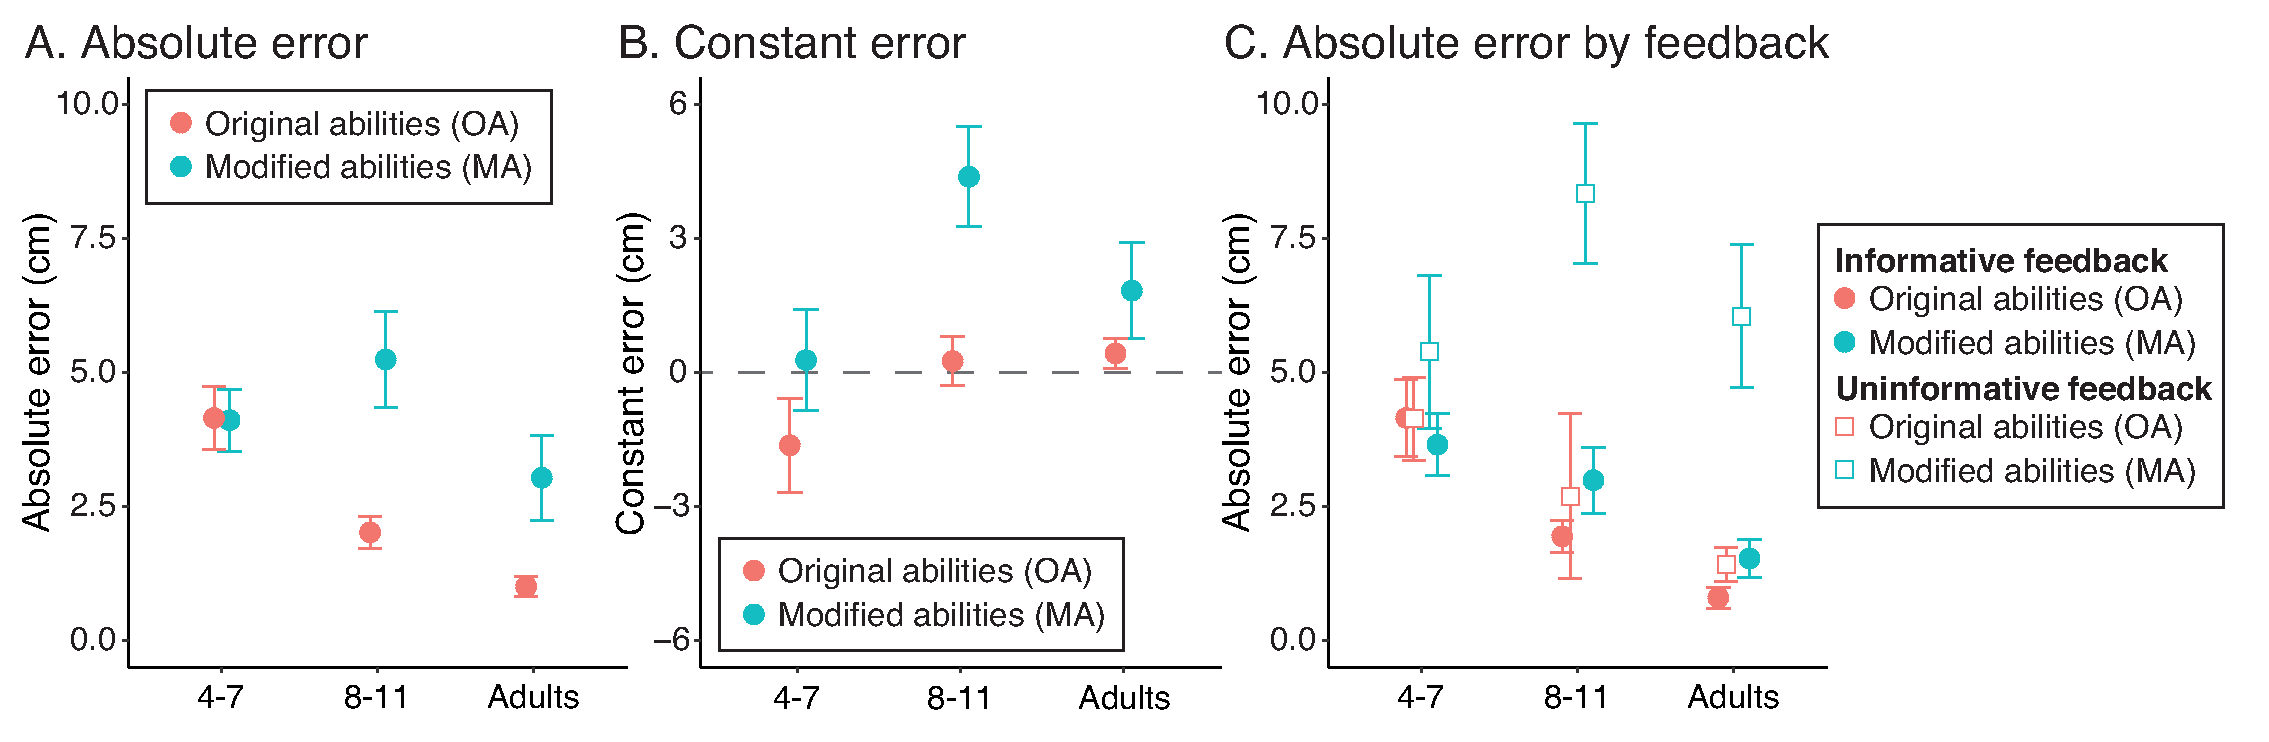
\includegraphics[width=1\textwidth]{error.eps}
\caption{\label{fig:error}(A) Absolute error and (B) constant error by age group and condition. Red symbols show the original ability condition and blue symbols show the modified abilities condition. (C) Absolute error by age group, condition, and feedback group. Circular symbols depict the informative feedback group and square symbols show the uninformative feedback group. Error bars show ± 1 SE.}
\end{figure}

\subsection{Constant error}

Figure \ref{fig:error}B shows that constant error increased with age and was greater for the MA condition compared with the OA condition. In the OA condition, younger children were biased towards selecting impossibly small doorways ($M$ = -1.63 cm, $SD = 4.72$); older children ($M$ = 0.25 cm, $SD$ = 2.45) and adults ($M$ = 0.42 cm, $SD$ = 1.14) were relatively unbiased. In the MA condition, more conservative judgments overall meant that younger children were unbiased ($M$ = 0.27 cm, $SD$ = 4.90) and that older children ($M$ = 4.38 cm, $SD$ = 4.87) and adults ($M$ = 1.82 cm, SD = 3.73) more often erred by saying “no” to doorways that were indeed possible to fit through. A 3 Age (younger children, older children, adults) × 2 Condition (OA, MA) permutation ANOVA confirmed significant mains effects of age ($p = .014, \eta^{2} = .10$) and condition ($p < .001, \eta^{2} = .09$), but the interaction was non-significant ($p = .35, \eta^{2} = .02$). The main effect of age was followed up by comparing each age group while collapsing across conditions. Younger children’s constant errors were significantly less compared with those of older children ($p$ = .006); however, no significant differences were found between younger children and adults ($p$ = .19) or between younger children and adults ($p$ = .25).

\subsection{Feedback and absolute error}

Participants were grouped based on their experiences during the decision trial block. The informative feedback (IF) group contained participants who experienced both success and failure experiences during the decision trial block, whereas the uninformative feedback (UF) group contained participants who received only success experiences, only failure experiences, or no experience during the decision trial block (Table \ref{tab:1}). 

\begin{table}
\caption{Absolute error (M and SD) and group size for participants in the informative feedback (IF) and uninformative feedback (UF) groups by age and condition.}
\label{tab:1}
\begin{tabular}{@{}lllllllll@{}}
\multicolumn{4}{c}{Informative Feedback (IF)}                                                                                   &                       & \multicolumn{4}{c}{Uninformative Feedback (IF)}                                                                  \\ 
\multicolumn{1}{l}{Condition} & \multicolumn{1}{l}{Age} & \multicolumn{1}{l}{\textit{M (SD)}} & \multicolumn{1}{l}{\textit{n}} & \multicolumn{1}{l}{} & \multicolumn{1}{l}{Condition} & \multicolumn{1}{l}{Age} & \multicolumn{1}{l}{\textit{M (SD)}} & \multicolumn{1}{l}{$n$} \\ \midrule
OA                              & 4-7                      & 4.1 (2.9)                            & 16                              &                       & OA                             & 4-7                      & 4.1 (1.6)                   & 4                      \\
OA                              & 8-11                     & 1.9 (1.3)                            & 18                              &                       & OA                             & 8-11                     & 2.7 (2.2)                   & 2                      \\
OA                              & Adults                   & 0.8 (0.5)                            & 8                               &                       & OA                             & Adults                   & 1.4 (0.6)                   & 4                      \\
MA                              & 4-7                      & 3.7 (2.2)                            & 14                              &                       & MA                             & 4-7                      & 5.4 (3.2)                   & 5                      \\
MA                              & 8-11                     & 3.0 (2.0)                            & 11                              &                       & MA                             & 8-11                     & 8.3 (3.7)                   & 8                      \\
MA                              & Adults                   & 1.5 (1.0)                            & 8                               &                       & MA                             & Adults                   & 6.0 (2.7)                   & 4                      \\ \bottomrule
\end{tabular}
\end{table}

Figure \ref{fig:error}C shows absolute error as a function of age, condition, and feedback type and reveals two striking results. First, only participants who received uninformative feedback struggled to recalibrate to modified abilities; there was no difference between MA and OA conditions for IF participants. Second, age-related improvements in accuracy were observed in both the MA and OA conditions for participants who generated informative feedback. These results were confirmed in a 3 Age (younger children, older children, adults) × 2 Condition (OA, MA) × 2 Feedback (IF, UF) permutation ANOVA on absolute error. As before (when feedback was not included in the model), the ANOVA revealed significant main effects of age ($p = .006, \eta^{2} = .10$) and condition ($p < .001, \eta^{2} = .15$) as well as a significant age × condition interaction ($p = .034, \eta^{2} = .06$). Furthermore, adding feedback to the model resulted in a significant feedback effect ($p < .001, \eta^{2} = .15$) and a significant condition feedback interaction ($p = .001, \eta^{2} = .10$). No other effects reached significance. 

To follow up on the age × condition and feedback × condition interactions, data were split by feedback group to run two separate 3 Age × 2 Condition permutation ANOVAs. For participants who generated informative feedback, the 3 Age × 2 Condition ANOVA revealed only a significant effect of age ($p < .001, \eta^{2} = .24$)---as Figure \ref{fig:error}C shows, the lines for the OA and MA conditions are superimposed and both decrease with age. Pairwise comparisons between age groups (collapsed across condition) confirmed that absolute error significantly differed between all three groups ($p$s < .016). Participants who experienced uninformative feedback showed a completely different pattern of results. The 3 Age × 2 Condition ANOVA revealed only a significant effect of condition ($p = .006, \eta^{2} = .33$)---indicating that participants perception of their original affordances were scaled regardless of feedback, recalibration to altered affordances depended on feedback regardless of age.

\section{Discussion}
Limitation = participant's error relates to whether they get feedback. In a way it's not a limitation because that's how it is in real life. But difficult to tease apart these things.

Future directions: compare recal in different types of tasks, better design for addressing how decisions to generate feedback relate to learning


\bibliography{example}


\end{document}

%
% Please see the package documentation for more information
% on the APA6 document class:
%
% http://www.ctan.org/pkg/apa6
%